\documentclass[fleqn,usenatbib]{mnras}
\usepackage[T1]{fontenc}
\usepackage{amsmath, mathtools}
\usepackage[dvipsnames]{xcolor}
\usepackage{pgfplotstable}
\pgfplotsset{compat=1.16}

\begin{document}

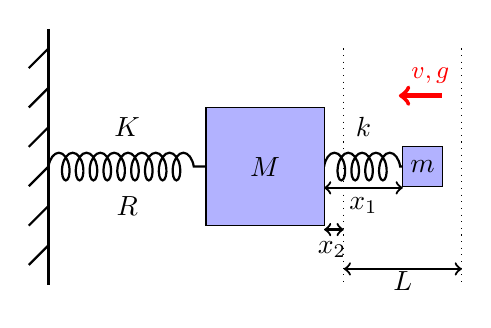
\begin{tikzpicture}
    % Spring NS
    \draw[thick,decorate,decoration={coil,amplitude=5, segment length=5}] (0,0) -- (2,0);
    % Spring clump
    \draw[thick,decorate,decoration={coil,amplitude=5, segment length=5}] (3.5,0) -- (4.5,0);
    % Mass NS
    \filldraw[fill=blue!30] (2,-0.75) rectangle (3.5,0.75);
    \node at (2.75,0) {$M$};
    % Mass clump
    \filldraw[fill=blue!30] (4.5,-0.25) rectangle (5.0,0.25);
    \node at (4.75,0) {$m$};
    % Wall: Centre of NS
    \draw[thick] (0,1.75) -- (0,-1.5);
    \foreach \y in {-1,-0.5,0,0.5,1,1.5} {
        \draw[thick] (0,\y) -- (-0.25,\y-0.25);
    }
    % Labels
    \node at (1,0.5) {$K$}; \node at (1,-0.5) {$R$};
    \node at (4,0.5) {$k$}; 
    \draw[<->, thick] (3.5,-0.27) -- (4.5,-0.27); \node at (4,-0.5) {$x_1$};
    \draw[<->, thick] (3.75,-1.3) -- (5.25,-1.3); \node at (4.5,-1.45) {$L$};
    \draw[<->, thick] (3.5,-0.8) -- (3.75,-0.8); \node at (3.6,-1.05) {$x_2$};
    % Direction of motion arrow
    \draw[<-, ultra thick, red] (4.45,0.9) -- (5.0,0.9);
    \node[red, font=\small] at (4.85,1.15) {$v, g$};
    % Zero line
    \draw[dotted] (3.75,1.5) -- (3.75,-1.5);
    \draw[dotted] (5.25,1.5) -- (5.25,-1.5);
\end{tikzpicture}

\end{document}